
\section{Representación gráfica de la serie de Fourier en una hoja de cálculo}

En la siguiente figura se representa un polinomio de cuarto grado en términos de `x'. Para graficar esta función en Excel, primero se eligen los valores de `x' para los cuales se desea evaluar la función. Luego, se calculan los valores correspondientes de `y' utilizando la expresión del polinomio. Estos pares de valores de `x' e `y' se organizan en dos columnas en Excel.

Una vez que se tienen los valores de `x' e `y', se seleccionan y se crea un gráfico de dispersión o de líneas en Excel. En este gráfico, los valores de `x' se colocan en el eje horizontal (eje x), mientras que los valores de `y' se colocan en el eje vertical (eje y).

\subsection{Figura 1. Función original}

En la figura 2, se muestran los valores de la función de acuerdo al cálculo que se efectuó.

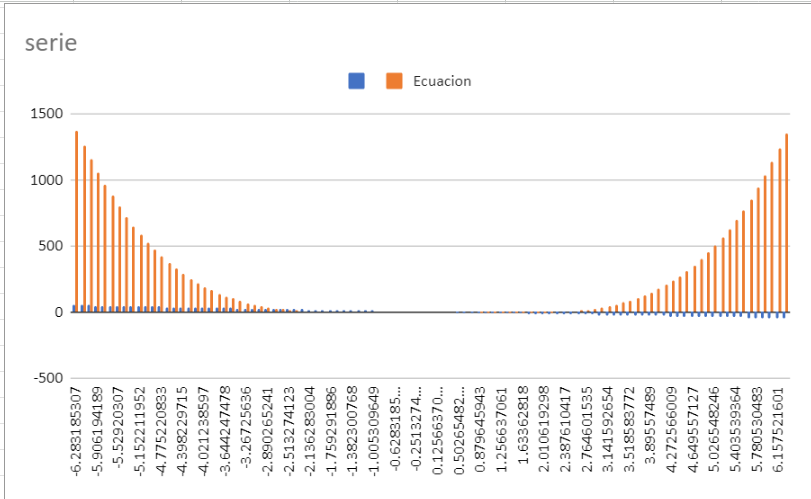
\includegraphics[width=6.26772in,height=3.44444in]{media/image10.png}

\subsection{Figura 2. Función original con valores calculados}

Finalmente en la \emph{Figura 3}, podemos observar y comparar las gráficas de la función por medio de los cálculos obtenidos a mano de la serie de Fourier, viendo la forma que toman y una similitud con la original que observamos en la \emph{Figura 1}.

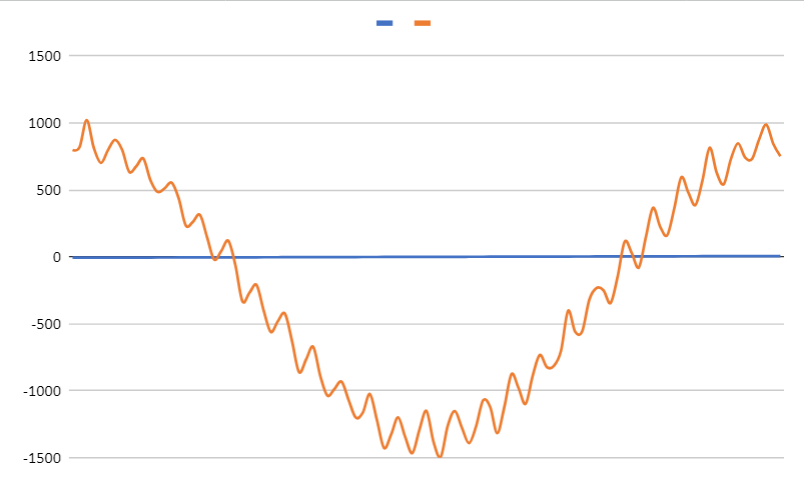
\includegraphics[width=5.10573in,height=3.08055in]{media/image16.png}

\subsection{Figura 3. Serie de Fourier aproximada en excel}
